%%%%%%%%%%%%%%%%%%%%%%%%%%%%%%%%%%%%%%%%%%%%%%%%%%%%%%%%%%%%%%%%%%
%%%%%%%% ICML 2015 EXAMPLE LATEX SUBMISSION FILE %%%%%%%%%%%%%%%%%
%%%%%%%%%%%%%%%%%%%%%%%%%%%%%%%%%%%%%%%%%%%%%%%%%%%%%%%%%%%%%%%%%%

% Use the following line _only_ if you're still using LaTeX 2.09.
%\documentstyle[icml2015,epsf,natbib]{article}
% If you rely on Latex2e packages, like most moden people use this:
\documentclass{article}

% use Times
\usepackage{times}
% For figures
\usepackage{graphicx} % more modern
%\usepackage{epsfig} % less modern
\usepackage{subfigure} 
\usepackage{amsmath,amsfonts,amssymb,bbm}
\usepackage{tikz}
\usetikzlibrary{fit,positioning}

% For citations
\usepackage{natbib}

% For algorithms
\usepackage{algorithm}
\usepackage{algorithmic}

% As of 2011, we use the hyperref package to produce hyperlinks in the
% resulting PDF.  If this breaks your system, please commend out the
% following usepackage line and replace \usepackage{icml2015} with
% \usepackage[nohyperref]{icml2015} above.
\usepackage{hyperref}

% Packages hyperref and algorithmic misbehave sometimes.  We can fix
% this with the following command.
\newcommand{\theHalgorithm}{\arabic{algorithm}}
\DeclareMathOperator{\Tr}{Tr}
\newcommand{\R}{\mathbbm{R}}
\newcommand{\mba}{\mathbf{a}}
\newcommand{\mbb}{\mathbf{b}}
\newcommand{\mbx}{\mathbf{x}}
\newcommand{\mbxt}{\tilde{\mathbf{x}}}
\newcommand{\Sigmat}{\tilde{\Sigma}}
\newcommand{\mbz}{\mathbf{z}}
\newcommand{\mbw}{\mathbf{w}}
\newcommand{\mcN}{\mathcal{N}}
\newcommand{\mcP}{\mathcal{P}}
\newcommand{\mcX}{\mathcal{X}}
\newcommand{\eps}{\epsilon}
\newcommand{\trans}{\intercal}
\newcommand{\Ut}{\tilde{U}}
\DeclareMathOperator*{\argmax}{arg\,max}
\newcommand{\angstrom}{\textup{\AA}}
\newcommand{\red}[1]{\textcolor{red}{[TODO: #1]}}


% Employ the following version of the ``usepackage'' statement for
% submitting the draft version of the paper for review.  This will set
% the note in the first column to ``Under review.  Do not distribute.''
%\usepackage{icml2015} 

% Employ this version of the ``usepackage'' statement after the paper has
% been accepted, when creating the final version.  This will set the
% note in the first column to ``Proceedings of the...''
\usepackage[accepted]{icml2015}


% The \icmltitle you define below is probably too long as a header.
% Therefore, a short form for the running title is supplied here:
\icmltitlerunning{Model of Quasar Spectroscopy}

\begin{document} 

\twocolumn[
\icmltitle{A Stochastic Process Model of Quasar Spectroscopy} %# \\
%Inference of Red Shift from Quasar Photometry }

% It is OKAY to include author information, even for blind
% submissions: the style file will automatically remove it for you
% unless you've provided the [accepted] option to the icml2015
% package.
\icmlauthor{Andrew Miller}{acm@seas.harvard.edu}
\icmlauthor{Albert Wu}{awu@college.harvard.edu}
\icmladdress{Harvard University,
             33 Oxford St, Cambridge, 02138 MA USA}
\icmlauthor{David Schlegel}{djschlegel@lbl.gov}
\icmladdress{Lawrence Berkeley National Laboratory, 
             1 Cyclotron Road, Berkeley, CA, 94720 USA}
\icmlauthor{Ryan Adams}{rpa@seas.harvard.edu}
\icmladdress{Harvard University,
             33 Oxford St, Cambridge, MA, 02138 USA}

             
% You may provide any keywords that you 
% find helpful for describing your paper; these are used to populate 
% the "keywords" metadata in the PDF but will not be shown in the document
\icmlkeywords{boring formatting information, machine learning, ICML}

\vskip 0.3in
]

\begin{abstract} 
We describe a method for combining information from two disparate sources of astronomical data, spectroscopy and photometry, which carry information about sources of light (e.g.~stars, galaxies, quasars) at extremely different resolutions. 
Our model treats the spectral energy distribution (SED) of the radiation of a source as a latent variable, hierarchically generating both photometric and spectroscopic observations.  
Furthermore, we view the problem of SED inference as a density estimation problem, placing a flexible nonparametric prior over the SED of a light source that admits a physically interpretable decomposition and allows us to tractably perform fully Bayesian inference using Markov chain Monte Carlo (MCMC).  
We use our model to predict the distribution of the redshift of quasars from five-band (low resolution) photometric data, the so called ``photo-z'' problem. 
Our method shows that tools from machine learning and Bayesian statistics can allow us to jointly model multiple resolutions of information to make accurate predictions with well-characterized uncertainties.  
%Our method leverages a small number of existing examples of high resolution quasar spectra with known redshift to build a structured prior distribution over unknown spectra.  
%We describe a fully generative model that combines information from a large dataset of high resolution spectroscopic measurements with a small number of broadband photometric observations, and we use it to measure the redshift of quasars from photometry, the ``photo-z'' problem.  
\end{abstract} 

\section{Introduction}
Enormous amounts of astronomical data are collected by a range of instruments at multiple resolutions, providing information about billions of sources of light in the observable universe~\cite{kent1994sdss, martin2005galex}.  
Among this collection of data are measurements of the spectral energy distribution (SED) of a source.  
The SED describes the distribution of energy radiated by a source over the spectrum of wavelengths or energy levels.  
For intuition, the SED of a star at around $5,800\, K$ (like our sun) radiates most of its energy in the $4,000 \angstrom$ to $7,000\angstrom$ range, which corresponds roughly to the range of visible light.  
However, stars tend to have simple distributions (well-modeled by Planck's law), whereas other objects, such as galaxies and quasars, can have much more complicated SEDs.  
The SED of a source is an object of interest because it carries information about the physical properties of the particular object, including type of source, effective temperature, distance to earth, and redshift. 

Measurements of SEDs, however, are produced by instruments at widely varying resolutions.  
Spectroscopic measurements can resolve noisy measurements of a source's SED in finer detail than broadband photometric measurements.  For example, the Baryonic Oscillation Spectroscopic Survey \cite{dawson2013baryon} measures SED samples at over four thousand wavelengths between 3,500 and 10,500 $\angstrom$.
In contrast, the photometry from the Sloan Digital Sky Survey (SDSS)~\cite{kent1994sdss} only gathers five broadband photometric measurements in the $u,g,r,i,$ and $z$ bands.  These measurements are the weighted-average response over a large swath of the wavelength spectrum, often expressed as a vector of band-specific fluxes, related to the number of photons measured over the duration of an exposure.  
The two methods of spectral information collection are graphically compared in Figure~\ref{fig:filters}. 

%------ SDSS Filter Figure -----------------------------------------------
\begin{figure*}[ht]
\vskip 0.2in
\begin{center}
\centerline{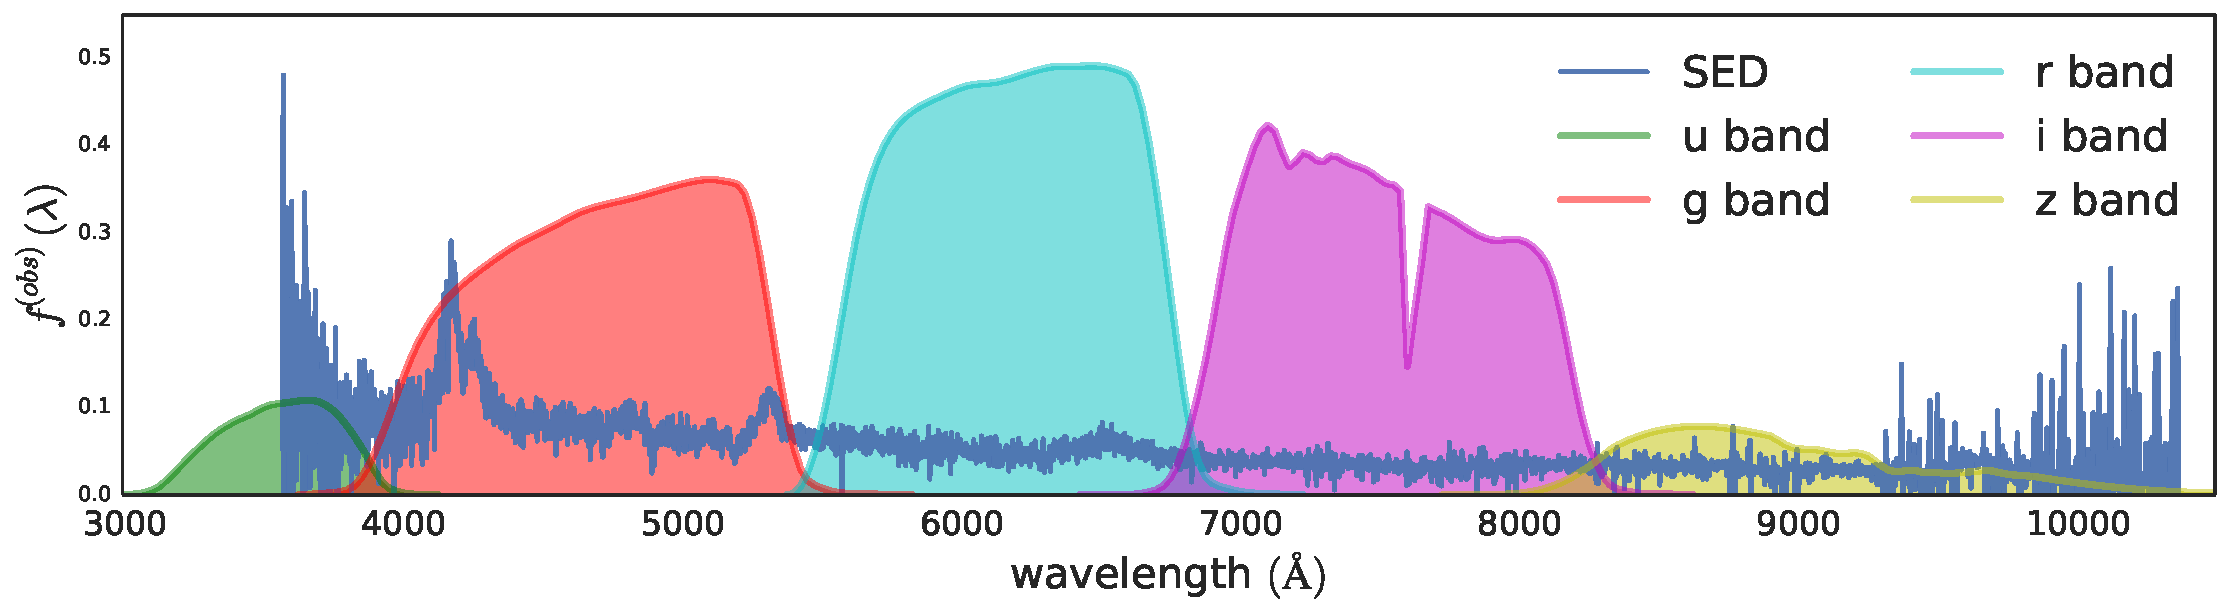
\includegraphics[width=2\columnwidth]{../figs/quasar_spectrum_sdss_filters}}
\caption{Example of a BOSS-measured quasar SED with SDSS \emph{ugriz} band filters, $S_{b}(\lambda)$, $b \in \{u, g, r, i, z\}$, overlaid.  Spectroscopic measurements include noisy samples at thousands of wavelengths, where as SDSS photometric fluxes reflect the (weighted) response over a large range of wavelengths.}
\label{fig:filters}
\end{center}
\vskip -0.2in
\end{figure*} 
%--------------------------------------------------------------------------


%------ example of obs vs rest frame data --------------------------------------
\begin{figure*}[ht]
\vskip 0.2in
\begin{center}
\centerline{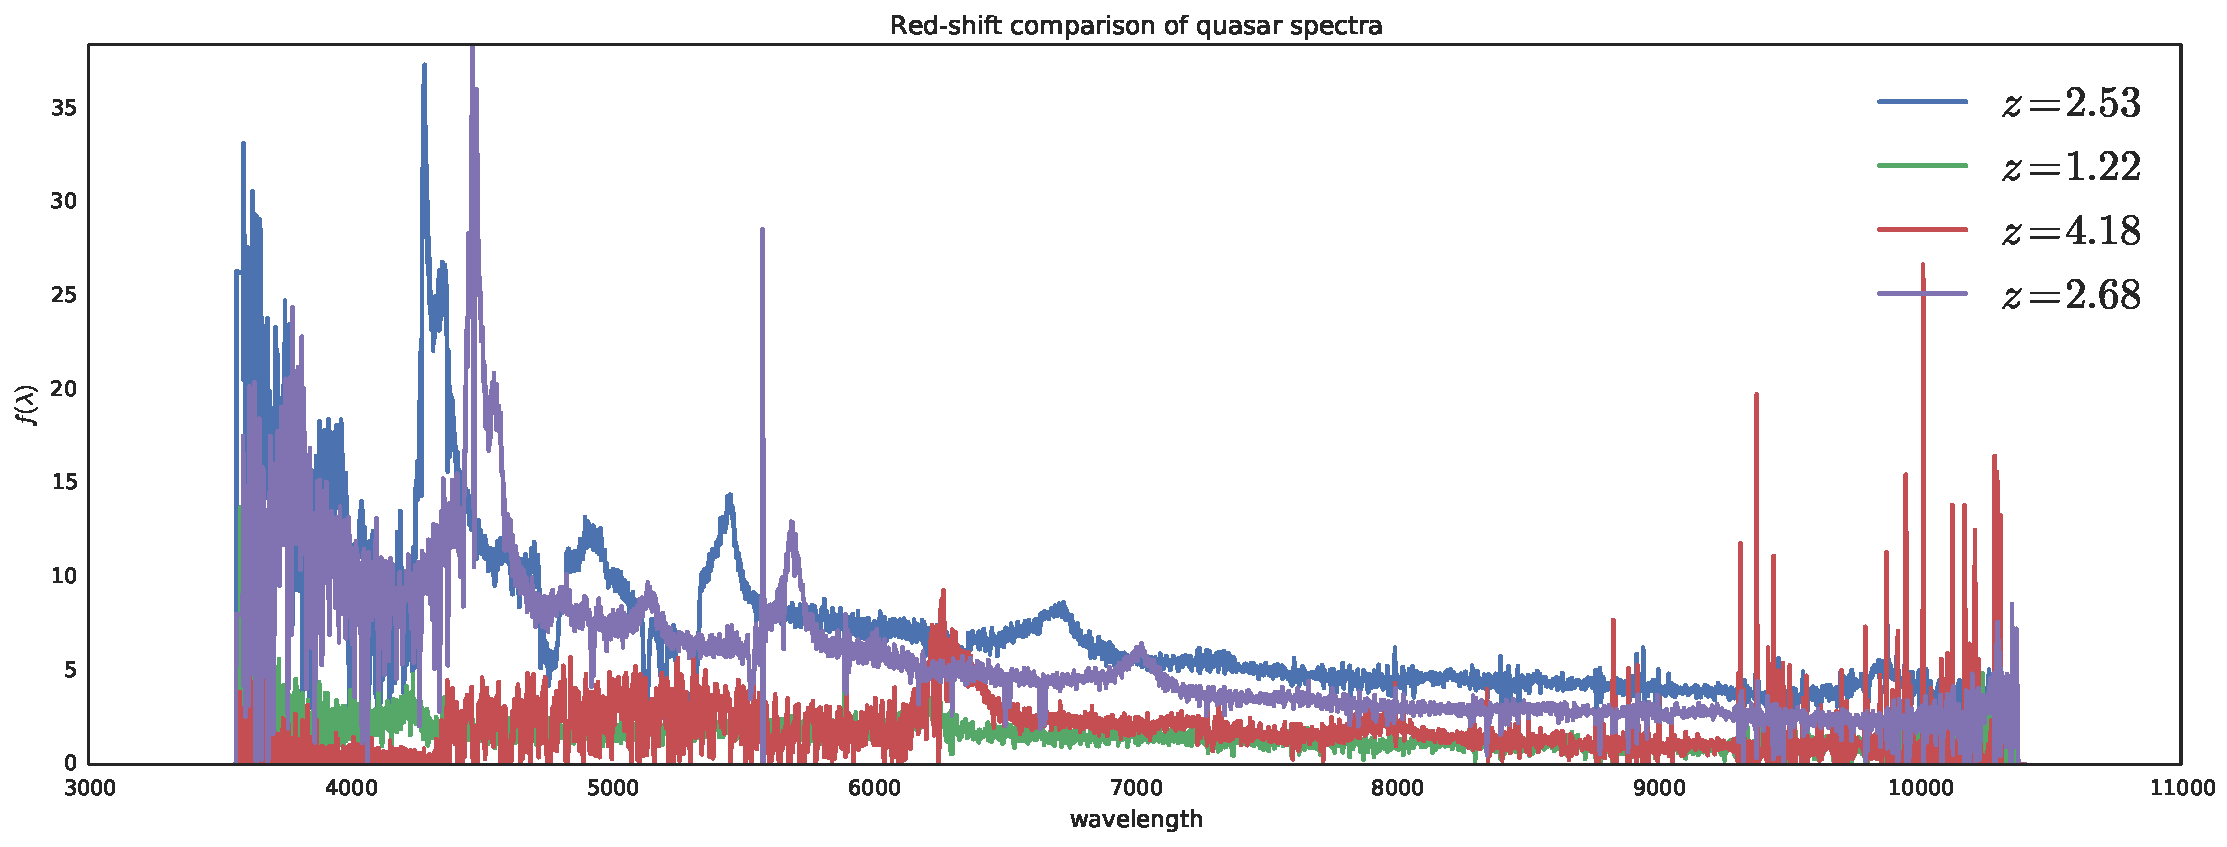
\includegraphics[width=2\columnwidth]{../figs/quasar_redshift_obs_frame}}
\centerline{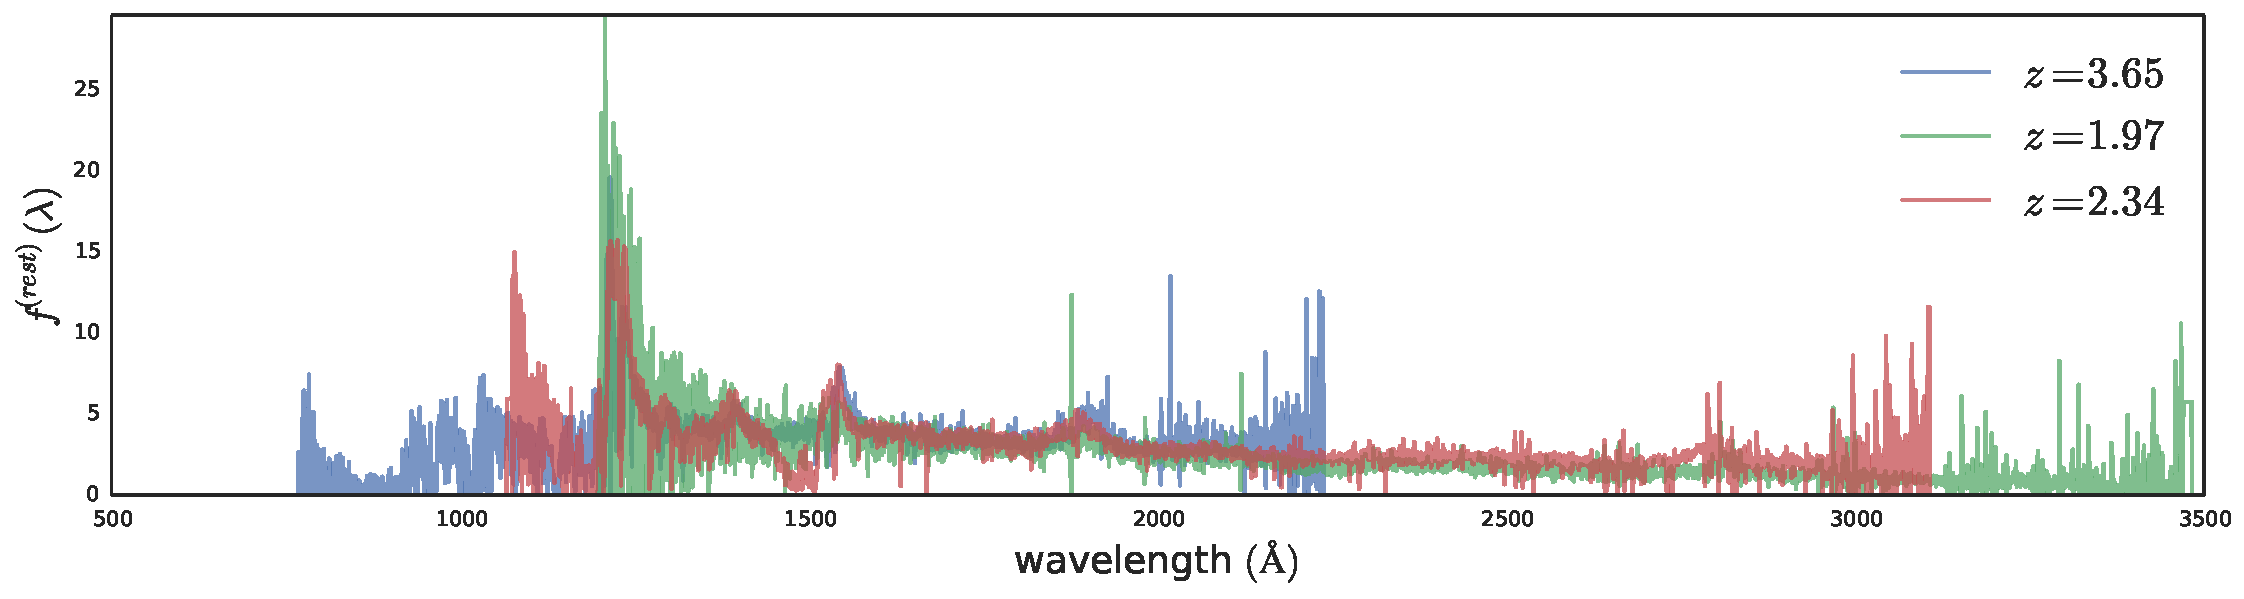
\includegraphics[width=2\columnwidth]{../figs/quasar_redshift_rest_frame}}
\caption{Spectroscopic measurements of multiple quasars at different redshifts, $z$.  The top graphic depicts the spectrograph in the observation frame, which can be intuitively thought of as ``stretched'' by a factor $(1+z)$.  The lower figure depicts the ``de-redshifted'' version of the same quasar spectra.  This effectively squashes observations, and reconstructs the quasar spectra as it would be seen in the quasar's rest frame.  The salient feature of this operation is the alignment of the emission and absorption lines (albeit at different scales).  This alignment will provide the information about $z$ that we can infer from SDSS photometric projections of the very same spectra.}
\label{fig:frames}
\end{center}
\vskip -0.2in
\end{figure*} 
%--------------------------------------------------------------------------------

Despite carrying less information, broadband photometric measurements are more widely available and exist for a larger number of sources than spectroscopic measurements. 
This work develops a method for extracting information from observations of light sources by \emph{jointly} modeling spectroscopic and photometric data.  
In particular, we use our model to measure the redshift of quasars for which we only have photometric observations.  
Redshift is a phenomenon in which the SED of a source of light is stretched toward longer (redder) wavelengths.  This effect can be caused by the source rapidly moving away from the observer (analogous to the Doppler effect) or due to the expansion of the universe \red{cite something here}.  
Quasars, or quasi-stellar radio sources, are extremely distant and energetic sources of electromagnetic radiation that can exhibit high redshift \red{cite something here}.  
Estimates and accurate characterization of uncertainty of redshift measurements from photometry have the potential to guide the study of certain quasars with higher resolution instruments.  
Furthermore, accurate models can aid the automation of identifying and classifying faintly observed quasars in large photometric surveys.  
%Identifying and measuring the redshift of a quasars from photometric data is a necessary task due to the widespread availability of large photometric surveys.  

%Study of distant quasars allow astronomers to observe the universe as it was many billions of years ago \red{need lots of references.}. 
Our model jointly describes both high-resolution spectroscopic data and low-resolution photometric observations of quasars in terms of their latent SEDs, luminosity, and redshift.  We represent a quasar's spectral energy as a latent variable, and describe a fully-Bayesian inference procedure to compute the marginal probability distribution of a quasar's redshift given observed photometric fluxes and their uncertainties.  The following section provides relevant application and statistical background, as well as related work on the ``photo-z'' problem.  Section~\ref{sec:model} describes our probabilistic model of SEDs and broadband photometric measurements.  Section~\ref{sec:inference} outlines our MCMC-based inference method for efficiently computing statistics of the posterior distribution. Section~\ref{sec:experiments} presents redshift and SED predictions from photometric measurements, among other model summaries.  We conclude with a discussion and directions for future work.  

\section{Background}
\label{sec:background}
The SED of an object describes the distribution of energy it radiates as a function of wavelength.  
For example, most stars are well-modeled as ideal blackbody radiators, so their SED closely follows Planck's law, which describes a parametric form for the spectral energy distribution. 
Quasars, on the other hand, have a complicated spectral energy distribution characterized by some salient features (\red{mention Ly-$\alpha$ and Ly-$\alpha$ forest?}).

Furthermore, quasars can be much more luminous and at a much higher redshift than stars and galaxies.  
Redshift affects our observation of SEDs by stretching the input space of wavelengths, $\lambda \in \Lambda$, of the quasar's \emph{rest-frame} SED.  
This skews the mass of the distribution toward longer (redder) wavelengths. Denoting the \emph{rest-frame} SED of a quasar $n$ as a function, $f_n^{(\text{rest})} : \Lambda \rightarrow \R_+$, the effect of redshift on the \emph{observation-frame} SED is summarized by the relationship 
\begin{align}
  f_n^{(\text{obs})}(\lambda) &\propto f_n^{(\text{rest})}(\lambda \cdot (1 + z_n)) \, .
\end{align}
Observed quasar spectra and their ``de-redshifted'' rest frame spectra are depicted in Figure~\ref{fig:frames}.

\subsection{Gaussian processes}
Due to the complicated form of observed spectroscopic data, we appeal to Gaussian process priors to flexibly encode our prior beliefs about the structure and shape quasar SEDs. 
A Gaussian process (GP) is a stochastic process, $f: \mathcal{X} \rightarrow \R$, such that any finite collection of random variables, ${f(x_1),\dots, f(x_N) \in \R}$, is distributed according to a multivariate normal distribution.  
GPs are frequently used as priors over unknown functions, $f$, where the random variables $f(x_1), \dots, f(x_N)$ correspond to evaluations of the function at inputs $x_1, \dots, x_N \in \mcX$.  
The prior covariance between any two points, $f(x_i)$ and $f(x_j)$, encodes prior beliefs about the function~$f$; carefully chosen covariance functions can encode beliefs about a wide range of properties, including differentiability, smoothness, and periodicity.  

Throughout this paper we will use the the Mat\'{e}rn \cite{Matern1986spatial} covariance function
\begin{align}
  k_{\text{Matern}}(r)(x_1, x_2) 
    &= \frac{2^{1-\nu}}{\Gamma(\nu)} 
       \left( \frac{\sqrt{\nu} r}{\ell} \right) ^\nu
       K_\nu\left( \frac{\sqrt{2\nu} r}{\ell}\right)
\end{align}
where $r = |x_1 - x_2|$.  Because this covariance is strictly a function of the distance between two points in the space $\mcX$, it is said to be stationary. 
See \cite{rasmussen2006gaussian} for a thorough treatment of Gaussian processes.  

\subsection{Related work}
Many machine learning and statistical methods have been applied to the ``photo-$z$'' problem. 
\citet{walcher2011fitting} divides ``photo-$z$'' methods into two categories, empirical methods and template-fitting methods.  Empirical methods are often discriminative, regression-based approaches, whereas template-fitting methods are often SED model-based approaches.  

A recent example of an empirical method uses a multi-layer perceptron with a combination of photometric datasets, including SDSS, 
%SDSS, UKIDSS, and WISE photometric fluxes datasets, 
to compute a regression function for redshift \cite{brescia2013photometric}. 
This method, while efficient and accurate in mean error, does not characterize the uncertainty of the estimated redshift, nor does it admit any physically interpretable estimate of the SED and quasar type.  

Template-based approaches use information derived from spectroscopically measured quasars to assist redshift predictions.  
\citet{budavari2001photometric} and \citet{richards2001photometric} present a clustering algorithm for reconstructing quasar SEDs from photometric observations and templates derived from noisy spectroscopic measurements.  
Their method clusters quasars into individual template categories using a $K$-means-like update, relying on weighted template averages of noisy SED measurements.  

Instead of a pure clustering method, we use a non-negative factor analysis-like model to represent the latent structure of quasar SEDs and a continuous and low-dimensional range of quasar types.  
Furthermore, our method presents a fully probabilistic model of SEDs and a Bayesian inference procedure that integrates out uncertainty over all variables, including  latent templates, individual loadings, and apparent brightness, to measure redshift.    

Other models blur the line between regression-based and generative models.  \citet{bovy2012photometric} develops a method termed $XDQSOz$ to use a large dataset of astronomical objects to simultaneously infer redshift and classify quasars.  
They model the joint distribution over object type, fluxes, and redshift.  However, their method does not model SEDs themselves, nor the SED-to-flux generative process. 
%They do this by inferring a joint distribution over object type, fluxes, and redshift. In particular, they factor this joint distribution
%into one part that describes the distribution over star brightness, which involves binning based on a single-channel flux, and
%one part that describes the distribution of relative fluxes (as compared to this channel) and the redshift. The latter distribution
%is represented by a mixture of up to 60 Gaussians. 
%However, we see that, due to the
%binning, this approach is not fully probabilistic or Bayesian.

\citet{benitez2000bayesian} presents a thorough summary of Bayesian methods for photometric redshift estimation from spectral templates.  
\citet{budavari2009unified} unifies template-based and regression-based
approaches into a single probabilistic framework, distinguishing methods based on the assumptions they impose on probability distributions over photometric fluxes. 

%\red{Others to mention: }
%\cite{suzuki2006quasar} does unsupervised learning on the UV spectra of quasars using principal components analysis (PCA). Through this analysis, the authors found that 96\% of the total variance was accounted for by the first 3 spectral components. As a result, they created a classification scheme based on the first two component's coefficients that separates quasars into five different classes. This classification scheme allows researchers to understand quasars better from a qualitative perspective.
%\red{This doesn't seem that relevant. What do you think, Andy?}


%----------------------------------------------------------------------------------
%----------------------------------------------------------------------------------
%----------------------------------------------------------------------------------
\section{Model}

%--- Graphical Model ------------------------------------------
\begin{figure}

\tikzset{
  latentnode/.style={draw, minimum width=5mm, shape=circle, ultra thick, black},
  dagconn/.style={arrows=->, black, thick},
  plate/.style={draw, shape=rectangle, rounded corners=0.5ex, thick,
    minimum width=3.1cm, text width=3.1cm, align=right, inner sep=10pt, inner ysep=10pt,label={[xshift=-44pt,yshift=14pt]south east:#1}}
}

%\begin{figure}
\centering
\begin{tikzpicture}
\tikzstyle{main}=[circle, minimum size = 10mm, thick, draw =black!80, node distance = 12mm]
\tikzstyle{connect}=[-latex, thick]
\tikzstyle{box}=[rectangle, draw=black!100,label={[xshift=-14pt,yshift=14pt]south east:#1}]
  \node[main, fill = gray] (x) {$x_{n,\lambda}$};
  \node[main, fill=gray] (sigma) [below=of x] { $\sigma^2_{n,\lambda}$};
  \node[main, distance = 18mm] (w) [right=of x] {$\mathbf{w}_n$};
  \node[main, node distance = 5mm] (m) [below=of w] {$m_n$};
  \node[main, node distance = 5mm] (z) [below=of m] {$z_n$};
  \node[main, node distance = 18mm] (B) [above=of w] {$B_k$};
  \node[main] (ell) [left=of B] {$\ell, \nu$};
  \node[main, distance = 18mm, fill=gray] (y) [right=of w] {$y_{n,b}$};
  \node[main, fill=gray] (tau) [below=of y] {$\tau^2_{n,b}$};
  \path (B) edge [connect] (x)
           (B) edge [connect] (y)
           (w) edge [connect] (x)
           (w) edge [connect] (y)
           (m) edge [connect] (x)
           (m) edge [connect] (y)
           (z) edge [connect] (x)
           (z) edge [connect] (y)
           (sigma) edge [connect] (x)
           (tau) edge [connect] (y)
           (ell) edge [connect] (B) ;
    
  % draw plates
  \node[plate=, minimum width=26mm, inner sep=12pt, fit=(x) (sigma), label={[xshift=-34pt,yshift=14pt]south east:$\lambda \in \Lambda$}] (plate1) {};
  \node[plate=, minimum width=26mm, inner sep=12pt, fit=(y) (tau), label={[xshift=-73pt,yshift=16pt]south east:$b \in \{u,g,r,i,z\}$}] (plate1) {};
  \node[plate=, inner sep=15pt, fit=(B), label={[xshift=-15pt,yshift=14pt]south east:$K$}] (plate1) {};
  \node[plate, minimum width=31mm, minimum height=55mm, inner sep=4.4mm,draw=black!100, fit= (x) (sigma), label={[xshift=-29pt,yshift=14pt]south east:$N_{\text{spec}}$}] {};
  \node[plate, minimum width=31mm, minimum height=55mm, inner sep=4.4mm,draw=black!100, fit= (y) (tau), label={[xshift=-29pt,yshift=14pt]south east:$N_{\text{photo}}$}] {};
\end{tikzpicture}
%\end{figure}

\caption{Graphical model representation of the joint photometry and spectroscopy model.  The left shaded variables represent spectroscopically measured samples and their variances.  The right shaded variables represent photometrically measured fluxes and their variances. }
\label{fig:graphical}
\end{figure}


\label{sec:model}
This section describes the details of our joint probabilistic model of spectroscopic and photometric observations.  

\subsection{Stochastic Process Model of Spectra}
The SED of a quasar is a nonnegative valued function $f : \Lambda \rightarrow \R^+$, where $\Lambda$ denotes the range of wavelengths and $\R^+$ are nonnegative real-valued numbers.  However, quasar SEDs are highly structured, and we model this structure by imposing the assumption that each SED is a convex mixture of $K$ latent, positive basis functions (or templates). 
Following \citet{budavari2001photometric} we set $K = 4$.  We also note that this is the number of PCA components that have been shown to carry over 90\% of the variation of quasar spectroscopy~\citet{suzuki2006quasar}. 
This model assumes there are a small number of latent ``types'' and that each quasar can be described by a short vector of mixing weights over ``types''. 
Our model specifies a quasar's \emph{rest-frame} SED as a random measure. 
We place a log-Gaussian process prior on each of these basis functions, and a prior over positive-weight values for each quasar.  

The generative procedure for quasar spectra begins with a shared positive basis of normalized SEDs
that map wavelengths to positive numbers:
\begin{align}
  \beta_k(\cdot) &\sim \mathcal{GP}(0, K_\theta) \, , k=1, \dots, K\\
  B_k(\cdot) &= \frac{\exp(\beta_k(\cdot))}{\int_\Lambda \exp(\beta_k(\lambda)) d\lambda}   \, ,
\end{align}
where $K_{\theta}$ is the Mat\'{e}rn kernel and $B_k$ is a normalized version of
the $\beta_k$. These bases are then shared among all quasar SEDs.  For each quasar, $n$, the unobserved SED is distributed
\begin{align}
  \mathbf{w}_n &\sim p(\mathbf{w}) \, , \text{ s.t. } \sum_{w_k} w_k = 1  \\
  m_n  &\sim p(m) \, , \text{ s.t. } m_n > 0 \\
  f^{(\text{rest})}_n(\cdot) &= \sum_{k} w_{n,k} B_k(\cdot)\\
  \tilde f^{(\text{rest})}_n(\cdot) &= m_n \sum_{k} w_{n,k} B_k(\cdot)\label{eqn:restsed} \\
  z_n &\sim p(z)
\end{align}
where $\mathbf{w}_n$ mix over the latent types, $m_n$ is an overall apparent brightness, $f_n^{(\text{rest})}$ and $\tilde f_n^{(\text{rest})}$ are the normalized SED and scaled SED, respectively, and $z_n$ is the quasar's redshift.  The distributions $p(\mathbf{w})$ and $p(z)$ are prior distributions over weights and redshifts, respectively.  

Each positive SED basis function, $B_k$ is normalized to integrate to one, and each quasar's weight vector $\mathbf{w}_n$ also sums to one.  This allows us to interpret the $f^{(\text{rest})}_n(\cdot)$ function as a density, scaled by $m_n$, which we treat as a nuisance parameter and integrate out.  
\red{Todo: Warp input for varying lengthscale}.  

For each quasar $n$, we observe noisy samples of the redshifted and scaled spectral energy distribution at a grid of wavelengths $\lambda \in \{\lambda_1, \dots, \lambda_P \}$.  Our \emph{observation frame} samples are modeled
\begin{align}
  x_{n, \lambda} 
    &\sim \mathcal{N}\left( \frac{1}{(1 + z_n)} \tilde f_n^{(\text{rest})}( \lambda \cdot (1 + z_n) ), \sigma_{n,\lambda}^2 \right)
    \label{eq:spec} 
\end{align}
where $\sigma_{n, \lambda}^2$ is known measurement variance from the instruments
used to make the observations.
The BOSS spectra (and our rest-frame basis) are stored in units ergs/cm$^2$/s/$\angstrom$. 

\subsection{Photometric flux model }
Photometric data summarize the amount of energy observed over a large swath of the wavelength spectrum.  Roughly, a photometric flux measures (proportionally) the number of photons hitting the instrument's lens over the duration of an exposure, filtered by a band-specific sensitivity curve. 
We will express measurements of flux in nanomaggies \red{reference}, a linear unit of flux, in our model.

Photometric fluxes and measurement error derived from broadband imagery have been computed directly from pixels \cite{luptonsdss}.  
SDSS photometric data are measured in $ugriz$ bands, giving us a vector, $\mathbf{y}_n$, of five flux values and their variances, $\tau_{n, b}$ for $b \in ugriz$. 
Each band, $b$, measures photon observations at each wavelength in proportion to a known filter sensitivity, $S_{b}(\lambda)$. 
The filter sensitivities for the SDSS $ugriz$ bands are depicted in Figure~\ref{fig:filters}, with an example observation frame quasar SED overlaid.  The actual measured fluxes can be computed by integrating the full object's spectrum, $m_n \cdot f_n(\lambda)$ against the filters.  For a band $b \in \{u, g, r, i, z \}$
\begin{align}
  \mu_b(f_n^{(\text{rest})}, z_n) &= \int f^{(\text{obs})}_n(\lambda) S_b(\lambda) C(\lambda) d \lambda 
\end{align}
where $C(\lambda)$ is a conversion factor to go from the units of $f_n(\lambda)$ to nanomaggies \red{ write out the conversion }. We use $\mu_b$ to represent the full function from 
a rest spectrum and red shift to a band-specific flux. This projection onto SDSS bands results in five fluxes $y_{n,b}$, which are modeled as independent Gaussian random variables with known variance
\begin{align}
  y_{n,b} | \mathbf{w}_n, z_n, m_n, B &\sim \mathcal{N}( \mu_b(f_n^{(\text{obs})}, z_n), \tau_{n,b} ) \, .
\end{align}
Conditioned on the basis, $\{B_k\}$, we can represent $f_n^{(\text{rest})}$ with a low-dimensional vector.  Note that $f_n^{(\text{rest})}$ is a function of $\mathbf{w}_n, z_n, m_n, B$ (see Equation~\ref{eqn:restsed}), so we can think of $\mu_b$
as a function of $\mathbf{w}_n, z_n, m_n, B$. We overload notation, and re-write the conditional likelihood of photometric observations as
\begin{align}
    y_{n,b} | \mathbf{w}_n, z_n, m_n, B &\sim \mathcal{N}( \mu_b(\mathbf{w}_n, z_n, m_n, B), \tau_{n,b} ) \, .
   \label{eq:phot}
\end{align}
Intuitively, what gives us statistical traction in inferring the posterior distribution over $z_n$ is the structure learned in the latent basis $B$ - the features that corresponds to distinguishing bumps and dips in the SED.  

\subsection{Joint model}
Given a sample of $M$ noisy full spectra and their sample locations, $\mathbf{X} \equiv \{\mathbf{x}_m, \lambda^{(\text{obs})}_m \}_{m=1}^M$, and a set of $N$ photometric fluxes, $\mathbf{Y} \equiv \{\mathbf{y}_n\}_{n=1}^N$, our full likelihood in terms of $\{ \mathbf{w}_m, z_m, m_m \}_{m=1}^M, B_1, \dots, B_K, \{ \mathbf{w}_n, z_n, m_n \}_{n=1}^N$ is 
\begin{align*}
  L( \{ \mathbf{w}_m, &~z_m, m_m \}, \{ B_k \}, \{ \mathbf{w}_n, z_n, m_n\} )  \\
    = & \prod_{m=1}^M p( \mathbf{x}_m | \mathbf{w}_m, z_m, m_m, \{ B_k \})  \\
      & \times \prod_{n=1}^N p( \mathbf{y}_n | \mathbf{w}_n, z_n, m_n, \{ B_k \})
\end{align*}
where the probability distribution of the first term in the product is given by \ref{eq:spec}, and the distribution for the second term in the product is given by \ref{eq:phot}.  The joint distribution is depicted as a graphical model in Figure~\ref{fig:graphical}.

We express the joint prior distribution over weights $\mathbf{w}_n$, $\mathbf{w}_m$, and basis $\{B_k\}$ as:
\begin{align}
  p( \{ \mathbf{w}_m, z_m \}, &\{ B_k \}, \{ \mathbf{w}_n, z_n \} )  \\
    = & p(\{ B_k \}) p( \{ \mathbf{w}_m, z_m \} )  \\
      & p( \{ \mathbf{w}_n, z_n \} | \{ \mathbf{w}_m, z_m \} ) 
\end{align}
where we condition the photometric weights on the spectroscopically fit weights.  

%----------------------------------------------------------------------------------
%----------------------------------------------------------------------------------
%----------------------------------------------------------------------------------
\section{Inference}
\label{sec:inference}
The ``photo-z'' tasks requires that we compute posterior marginal distributions of $z$, $\mathbf{w}$, and $m$.  To compute these distributions, we construct an MCMC sampling algorithm that constructs a Markov chain over the state space including $z$, $\mathbf{w}$, $\mathbf{m}$, and $B$ that leaves the target posterior distribution invariant.  
 
For example, to compute expectations with respect to the marginal posterior distribution over quasar redshift, we will want to produce posterior samples of $z_n$, $\mathbf{w}_n$, and $B$
\begin{align}
  E[ g(z_n) | \mathbf{y}_n, \mathbf{X} ] 
    &\approx \sum_{i} g(z_n^{(i)}) \\
    z_n^{(i)}, \mathbf{w}_n | \mathbf{y}_n, B^{(i)} &\sim p(z_n, \mathbf{w}_n^{(i)} | \mathbf{y}_n, B^{(i)}) \\
    B^{(i)} &\sim p(B | \mathbf{X}) \, .
\end{align}

This section outlines our MCMC procedure to compute posterior samples of $\mathbf{w}_n, z_n, m_n$ and $B$ given the sample of spectra, $\mathbf{X}$, and photometric fluxes $\mathbf{y}_{ugriz}$.  Note that due to analytic intractability, we numerically integrate expressions $\int_\Lambda f_n^{(obs)}(\lambda) d\lambda$. 

\subsection{Sampling $B$}
To accelerate computation, we use only information present in $\mathbf{X}$ to draw samples of $B_1, \dots, B_K$.  That is, we approximate the full conditional distribution 
\begin{align}
  p(B_1,\dots, B_k | \mathbf{X}, \mathbf{Y}) 
    &\approx p(B_1, \dots, B_k | \mathbf{X})
\end{align}
We expect this to have little effect on the distribution, as the amount of information about $B$ present in $\mathbf{X}$, the high-resolution full-spectrum data, is expected to dwarf that of $\mathbf{Y}$, the
low-resolution bandwise fluxes.  The posterior distribution from which we sample, $p(B | \mathbf{X})$, can be written 
\begin{align}
  p(B | \mathbf{X}) 
    &\propto p(\mathbf{X} | \{ \mathbf{w}_m\}_{m=1}^M, B) p(\beta) p(\mathbf{w}) \, .
\end{align}
We draw posterior samples using Hamiltonian Monte Carlo \cite{neal2011mcmc}, an auxiliary variable method that uses gradient information to efficiently mix.  Empirically, naive Metropolis-Hastings mixes too slowly for practical purposes. 

\subsection{Sampling $\mathbf{w}_n, m_n$, and $z_n$}
Conditioned on a basis $B_k, k=1,\dots, K$, we can draw posterior samples of $\mathbf{w}_n$ and $z_n$ independently for each $n$
\begin{align}
  &p(\mathbf{w}_n, m_n, z_n | B, \mathbf{y}_n) \\
  &\propto p(\mathbf{y}_n | \mathbf{w}_n, m_n, z_n, B) p(\mathbf{w}_n, m_n, z_n) \\
  &= p(\mathbf{y}_n | \mathbf{w}_n, m_n, z_n, B) p(\mathbf{w}_n) p(m_n, z_n)
\end{align}
where our likelihood term is defined in Equation~\ref{eq:phot}. 

We place independent priors over $\mathbf{w}_n$, $m_n$, and $z_n$.  Again, we appeal to Hamiltonian Monte Carlo with an adaptive step size during burn-in to sample from this conditional \cite{neal2011mcmc}. 

%----------------------------------------------------------------------------------
%----------------------------------------------------------------------------------
%----------------------------------------------------------------------------------
\section{Experiments}
\label{sec:experiments}
We fit our model on a sample of 400 spectroscopic measurements from the the DR10QSO dataset \cite{paris2014sloan}, which includes spectroscopically confirmed redshifts from over 150,000 quasar spectra.  
We test our method by predicting redshift and SED of sample of 1,000 spectroscopically and photometrically measured quasars.  
We compute the posterior distribution by iterating our sampler over the conditional distributions described in the previous section.  For each of the 1,000 test quasars, we run 7 chains for 5000 iterations to assess mixing.  We discard the first 2,500 samples from each chain as burn-in.  The following subsections summarize and discuss model predictions and output.  

%------ Reconstructed quasar SEDs -----------------------------------------------
\begin{figure*}[th]
\vskip 0.2in
\begin{center}
\centerline{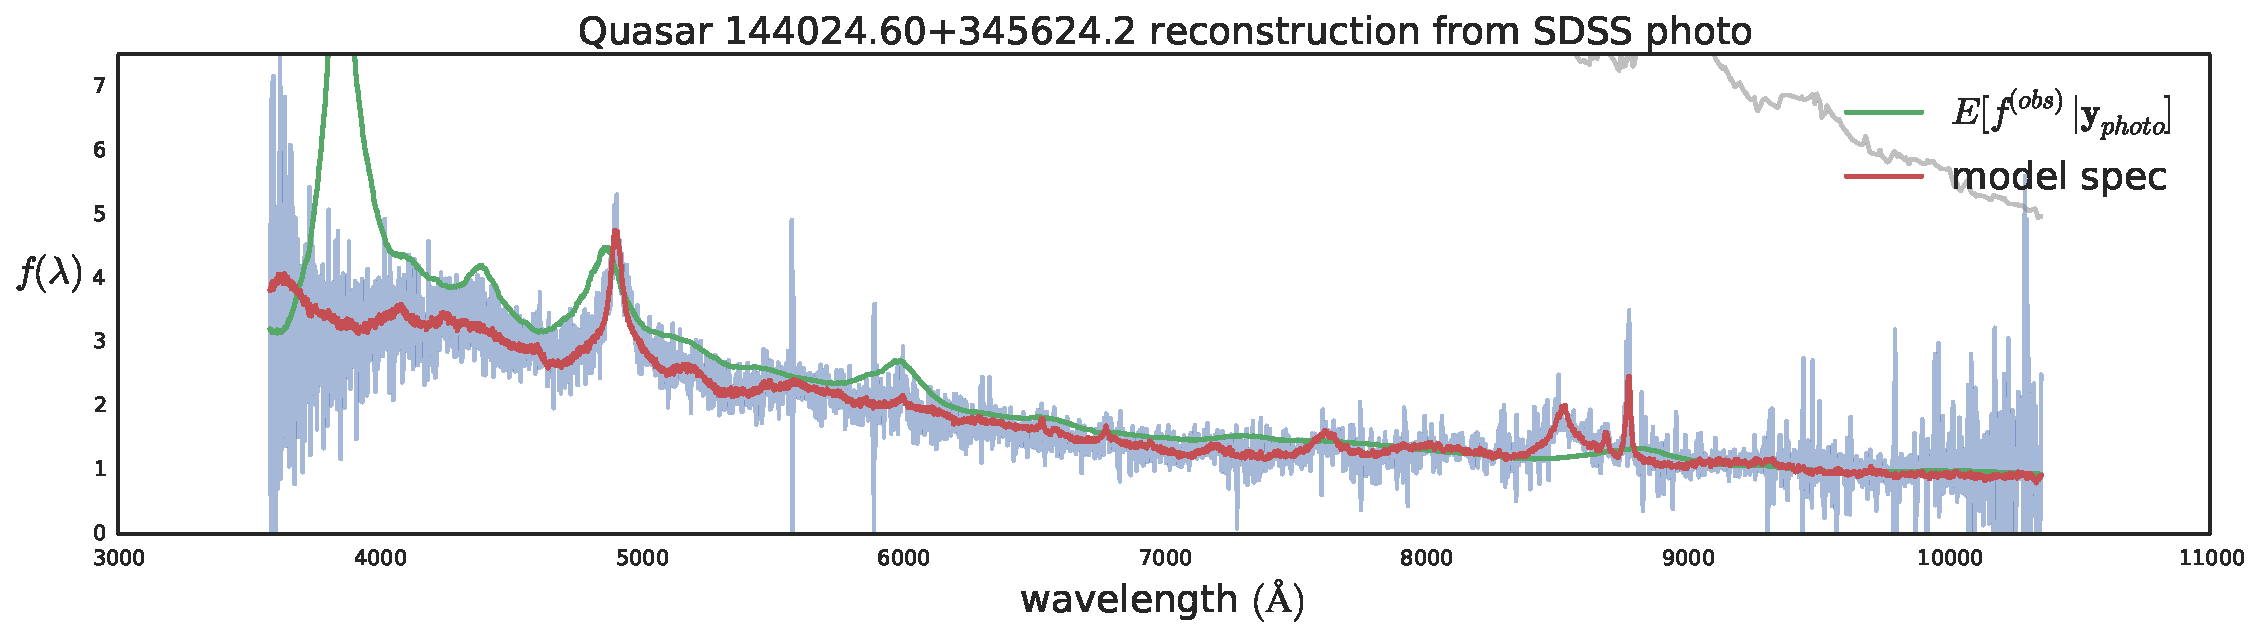
\includegraphics[width=2\columnwidth]{../figs/quasar_plots/quasar_56_mcmc_recon.pdf}} 
\centerline{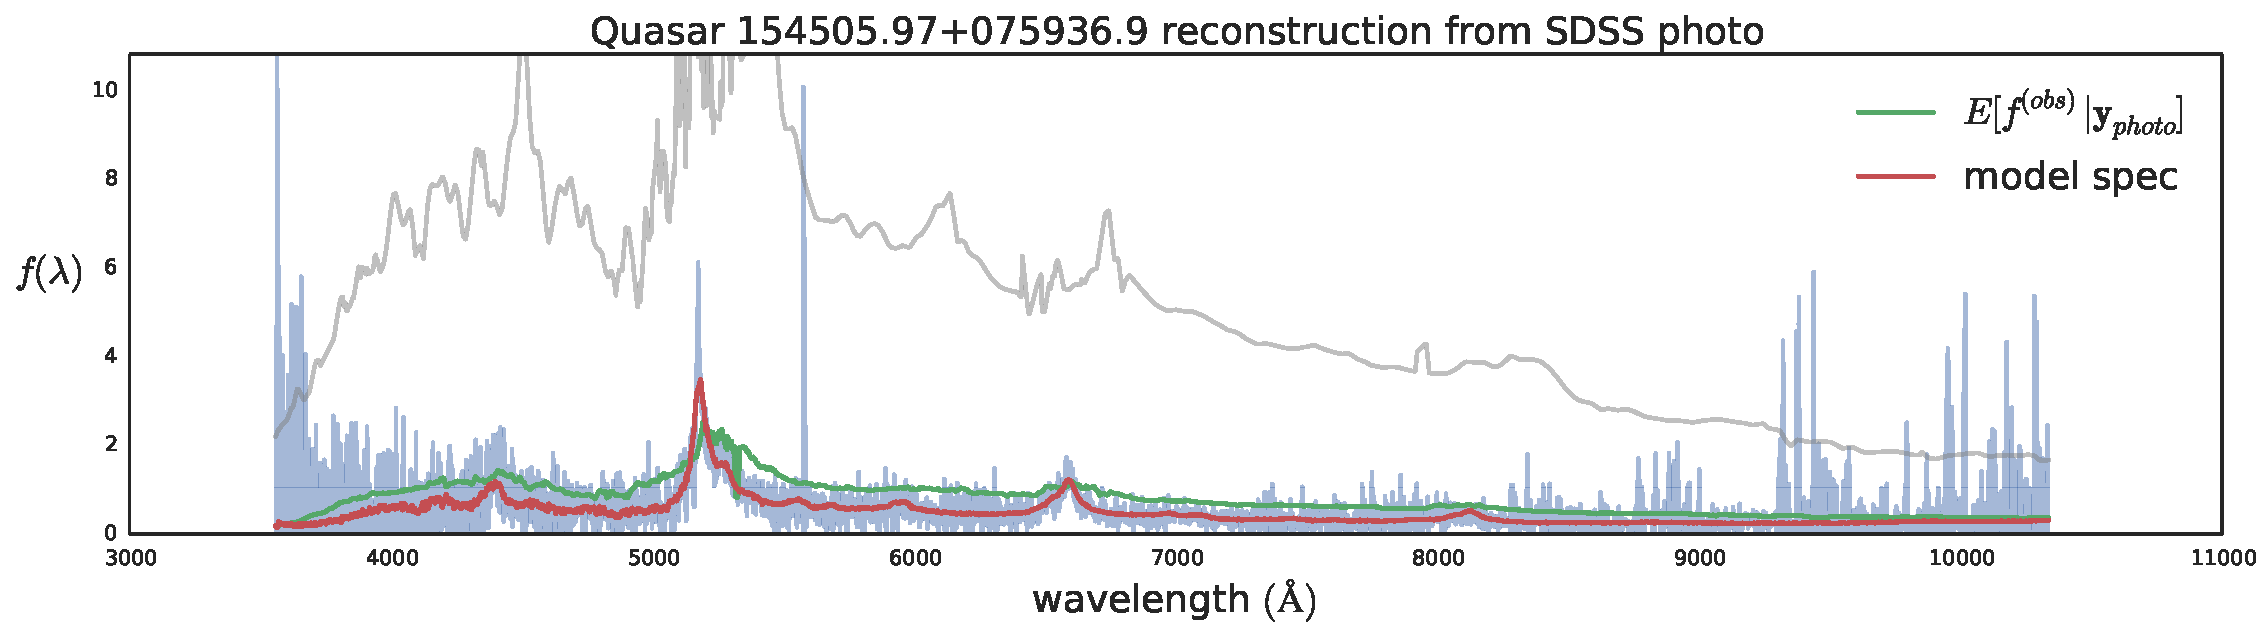
\includegraphics[width=2\columnwidth]{../figs/quasar_plots/quasar_119_mcmc_recon.pdf}} 
\vskip -0.2in
\caption{Inferred SEDs from photometric data.  The red line is a PCA-based model fit to the full spectral data.  The green line is the posterior median of $f^{(obs)}_n(\lambda)$. }
\label{fig:recon}
\end{center}
\end{figure*}
%-------------------------------------------------------------------------------

%----- Red Shift, spec vs photo -------------------------------------------------
\begin{figure}[h]
\vskip 0.2in
\begin{center}
\centerline{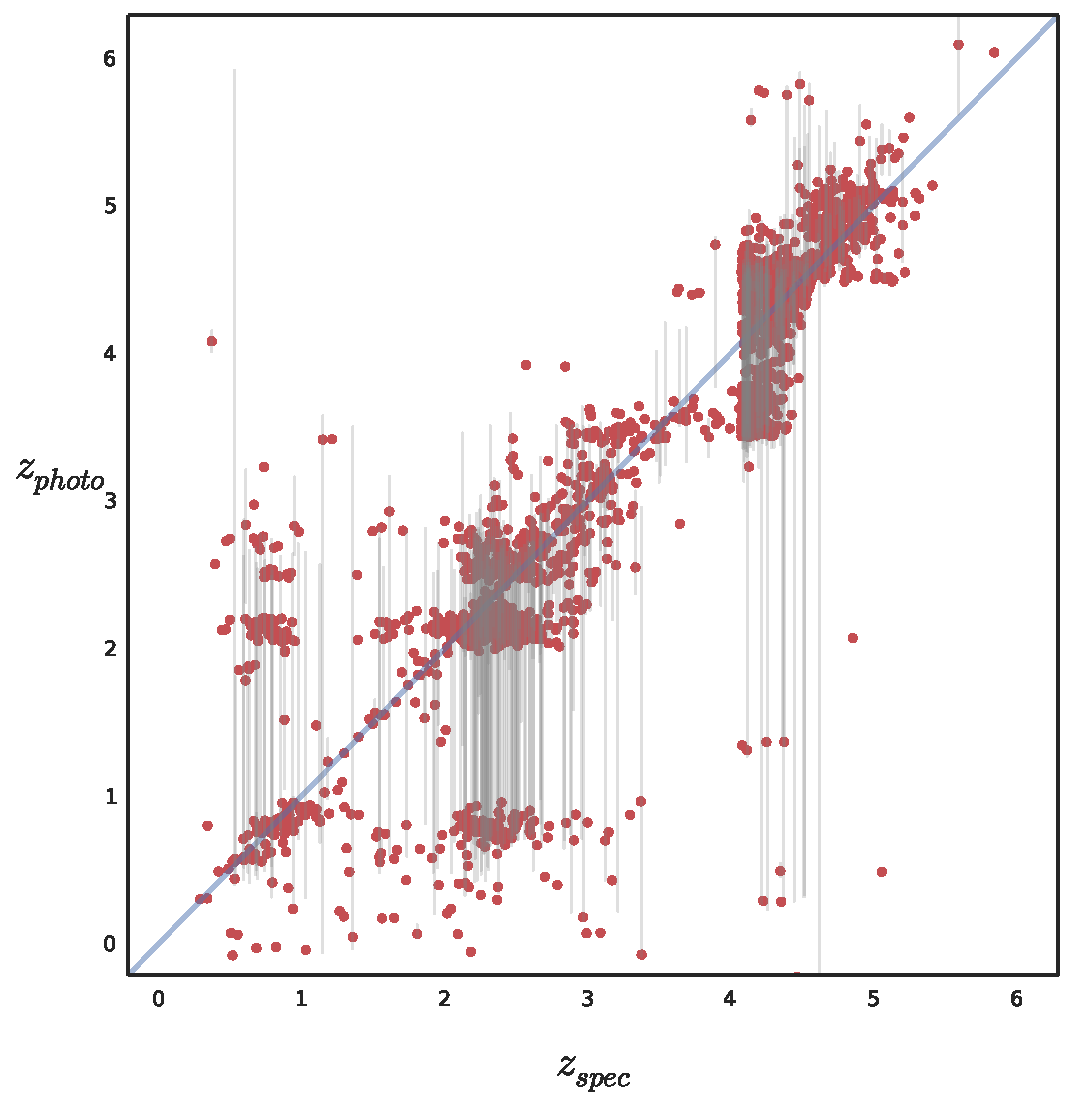
\includegraphics[width=\columnwidth]{../figs/red-shift-test-predictions}}
\vskip -0.2in
\caption{Comparison of spectroscopically ($x$-axis) and photometrically ($y$-axis) measured redshifts for a held out sample of 1,000 quasars.  Red estimates are the posterior mean $E[z_n | \mathbf{y}_n, \mathbf{X}]$, and grey lines display the the 99\% credible interval consisting of samples within quantiles $(.05, .995)$.  The estimate of each quasar is based on 750 samples from five HMC chains, after discarding 750 ``burn-in'' samples. }
\label{fig:vs}
\end{center}
\end{figure}
%-------------------------------------------------------------------------------


\subsection{Spectroscopic vs.~photometric measurements}

Using information only from $M = 400$ noisy high resolution SED measurements, our structured prior is able to accurately predict and characterize uncertainty about the redshift of photometrically measured quasars.  
Figure~\ref{fig:vs} compares our photometrically measured redshifts to spectroscopic measurements.  
\red{ address over-prediction cluster below $z_{spec} = 1$.  Is it because of our discretization of the basis?  Is it because of some information loss in that range due to the SDSS filter sensitivities/ranges?  Is it because our inference procedure is failing to find a better solution?}

We display marginal redshift distributions for individual quasars in Figure~\ref{fig:marginals}, and compare the value of the expected posterior to the spectroscopically measured redshift. 

Furthermore, because we are directly modeling the latent SED, our method admits a probabilistic estimate of the entire SED sample path conditioned only on observed photometric fluxes.  Figure~\ref{fig:recon} displays spectroscopic measurements of test-set quasars for which we inferred SEDs from only SDSS photometric measurements.  

We also quantify average prediction error and posterior credible interval coverage for sets of quasars with increasing redshift.  We see that our method is quite successful for quasars with redshift higher than 1, measuring within $.25$ of the spectroscopically confirmed redshift, and an average error of $11 \%$ or less.  More details are listed in Table~\ref{tab:error}. 

\subsection{Quasar types}
Our sampler yields posterior samples of the templates themselves; one sample is depicted in Figure~\ref{fig:basis}.  The loadings of individual quasars onto these bases intuitively describe the ``type'' of quasar being modeled.  \red{Visualize $w_n$ clusters and look at individual types. Show utility of this decomposition}.  Furthermore, because we restrict the templates to be positive functions, we obtain a more physically interpretable clustering of quasars than PCA-based methods, which will have both negative principal components and negative weights.  

\red{Discuss more informative prior on $w_n$ values} 

%----- Red Shift, spec vs photo -------------------------------------------------
\begin{figure*}[t]
\vskip 0.2in
\begin{center}
\centerline{
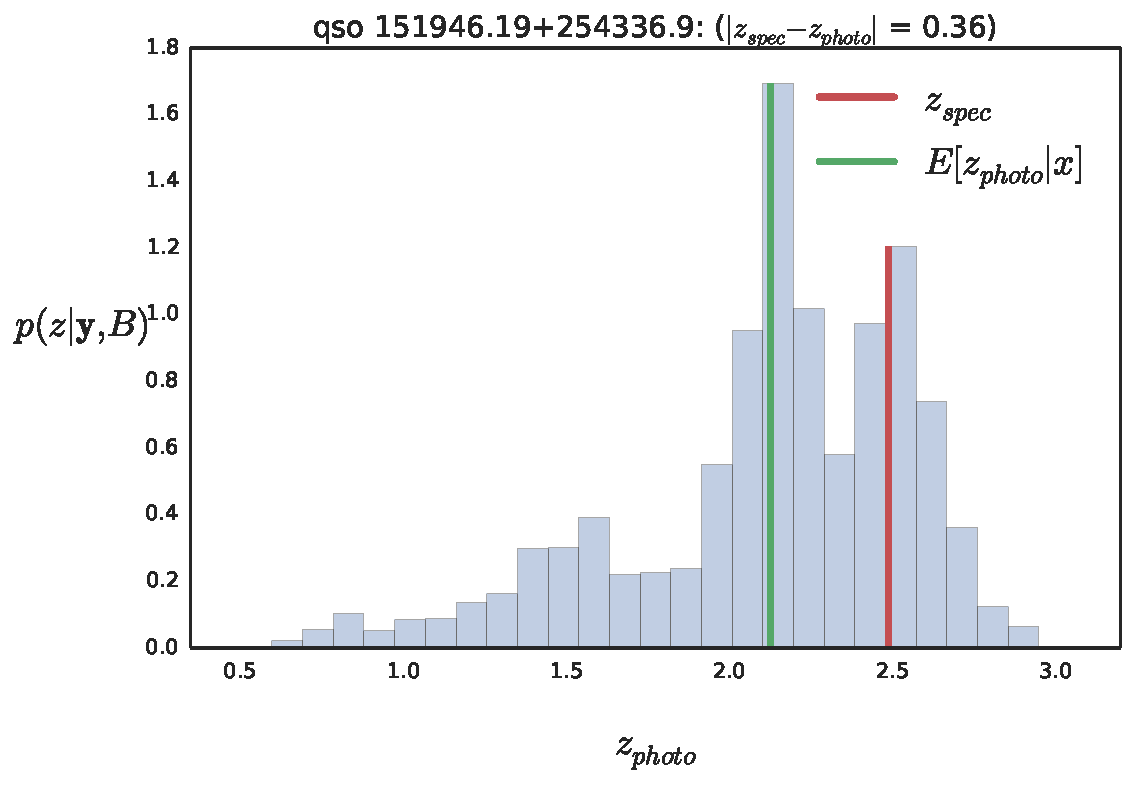
\includegraphics[width=.66\columnwidth]{../figs/quasar_plots/quasar_94_posterior_z}
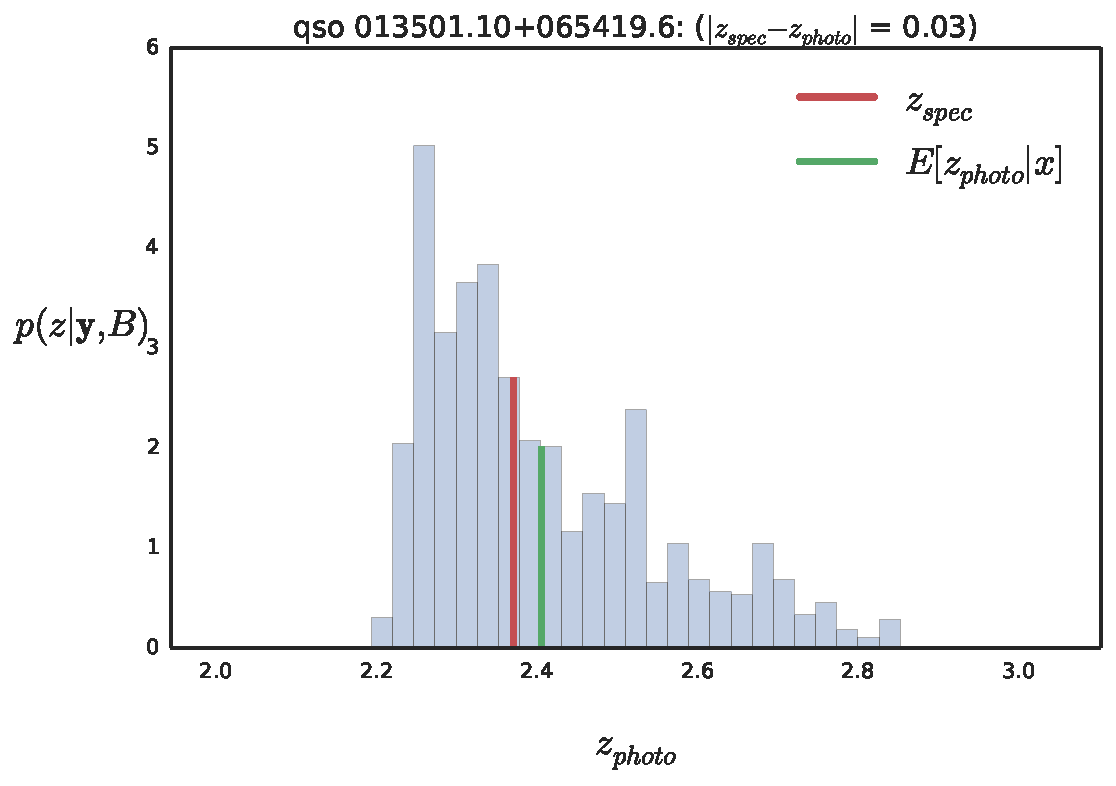
\includegraphics[width=.66\columnwidth]{../figs/quasar_plots/quasar_49_posterior_z}
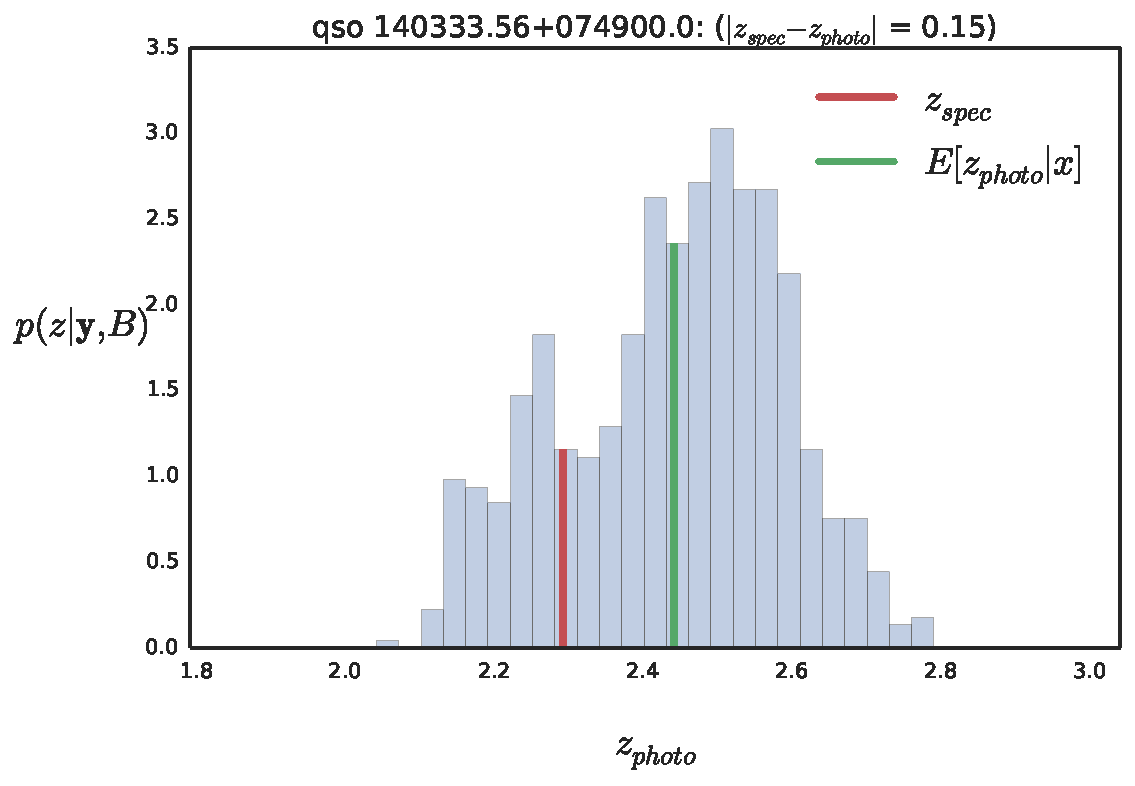
\includegraphics[width=.66\columnwidth]{../figs/quasar_plots/quasar_22_posterior_z}
}
\vskip -0.2in
\caption{Posterior predictive distributions, $p(z_n | \mathbf{X}, \mathbf{y}_n)$ for three photometrically measured quasars. The red-line is the spectroscopically confirmed redshift, and the green line is the posterior mean $E(z_n |\mathbf{X}, \mathbf{y}_n)$ }
\label{fig:marginals}
\end{center}
\end{figure*}
%---------------

%----- Red Shift, spec vs photo -------------------------------------------------
\begin{figure*}[t]
\vskip 0.2in
\begin{center}
\centerline{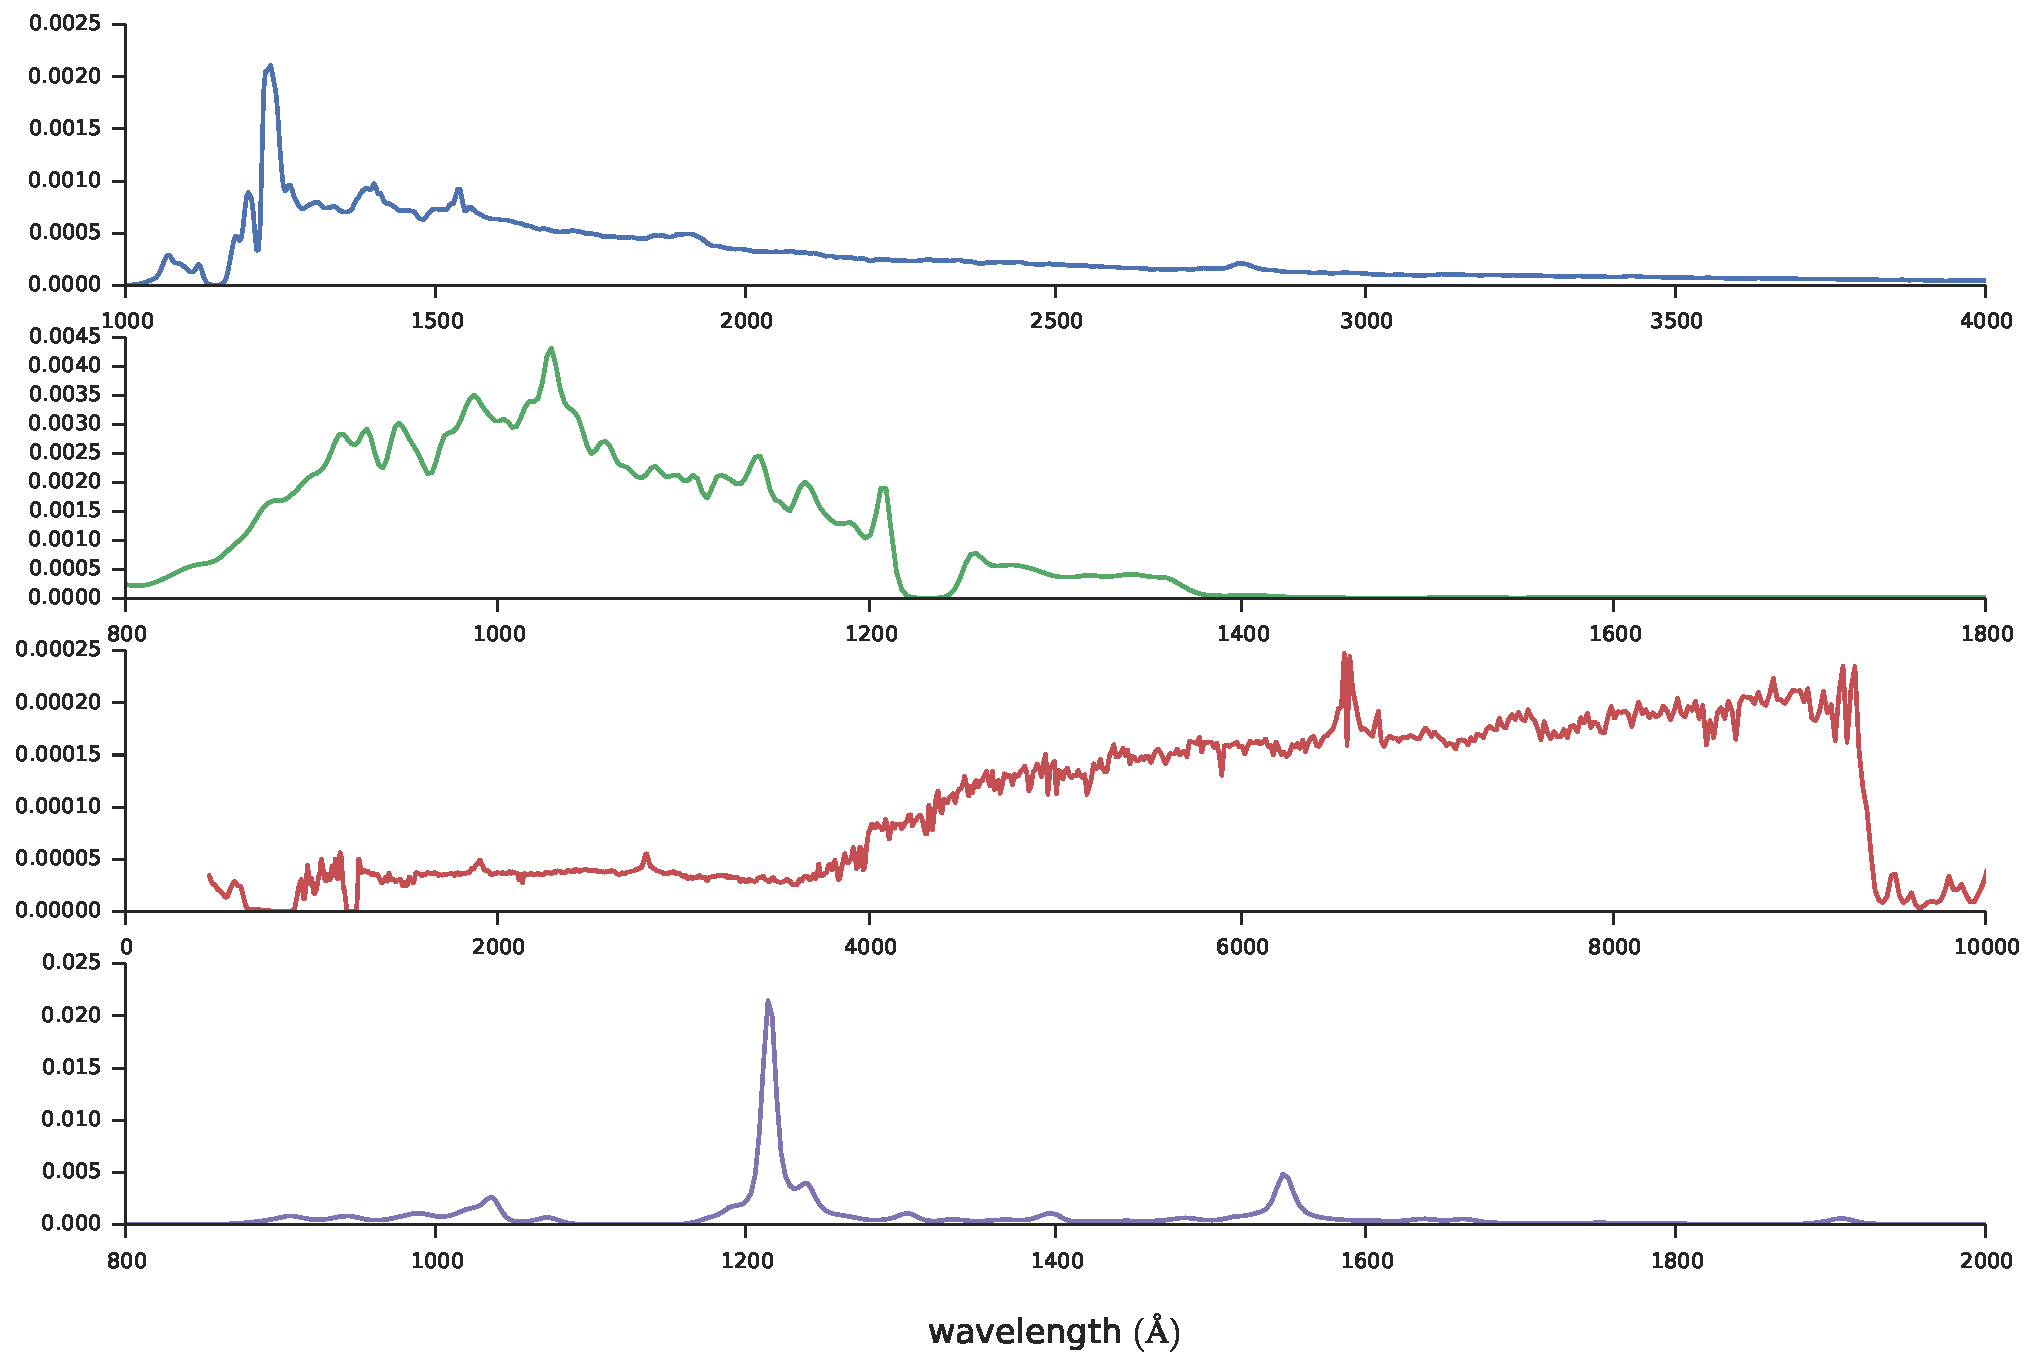
\includegraphics[width=2\columnwidth]{../figs/basis_samp_K_4}}
\vskip -0.2in
\caption{A posterior sample of the basis $\{ B_k \}_{k=1}^K$ for $K=4$.  Note the different ranges of the $x$-axis (wavelength).  Each basis function distributes its mass across different regions of the spectrum to explain different salient features of quasar spectra in the rest-frame. }
\label{fig:basis}
\end{center}
\end{figure*}
%---------------

%----- Red Shift, spec vs photo -------------------------------------------------
\begin{figure*}[t]
\vskip 0.2in
\begin{center}
\centerline{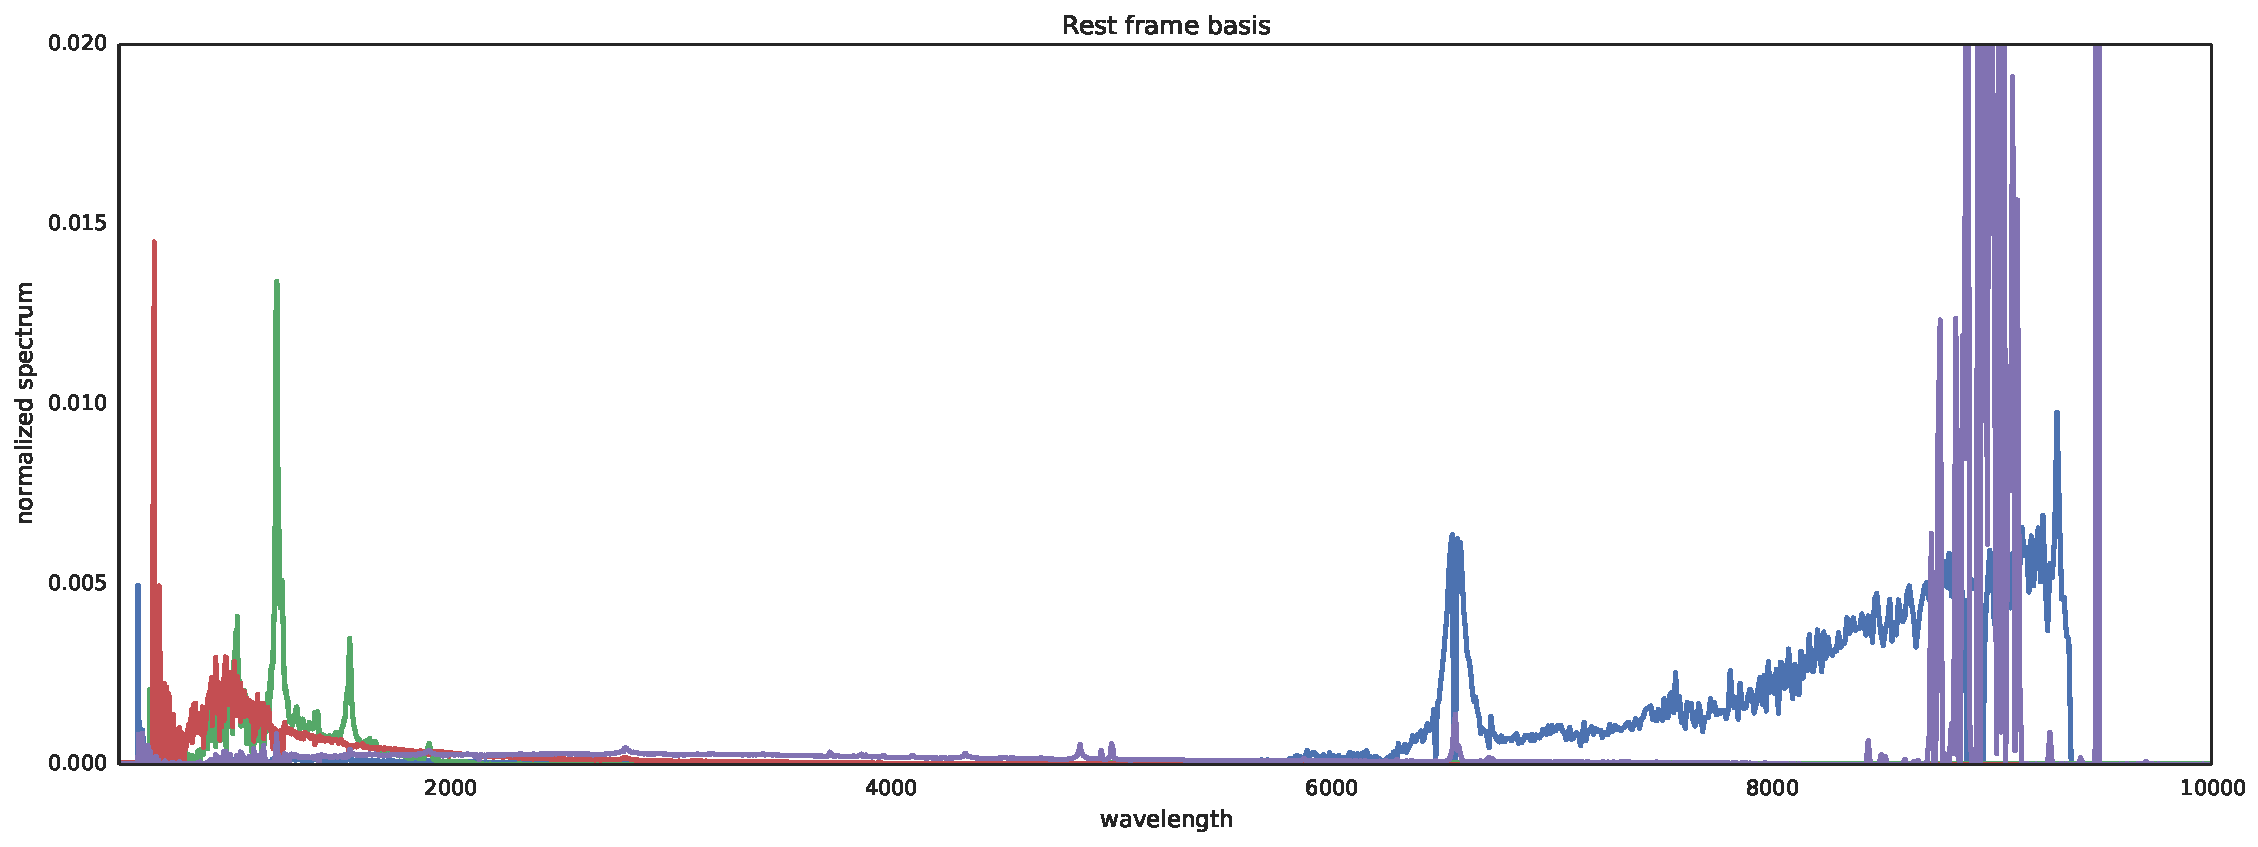
\includegraphics[width=2\columnwidth]{../figs/rank_4_basis}}
\centerline{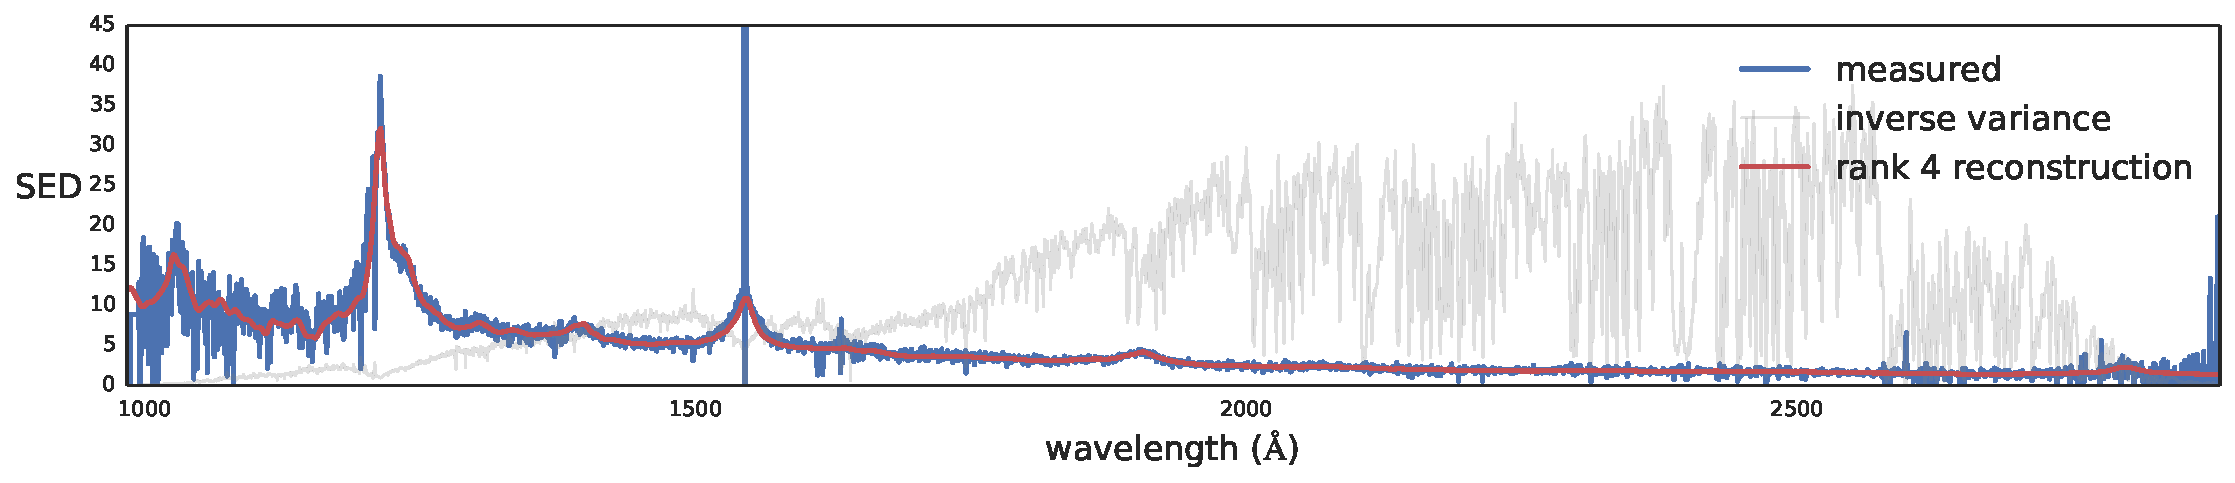
\includegraphics[width=2\columnwidth]{../figs/idx_0_rank_4_reconstruction.pdf}}
\centerline{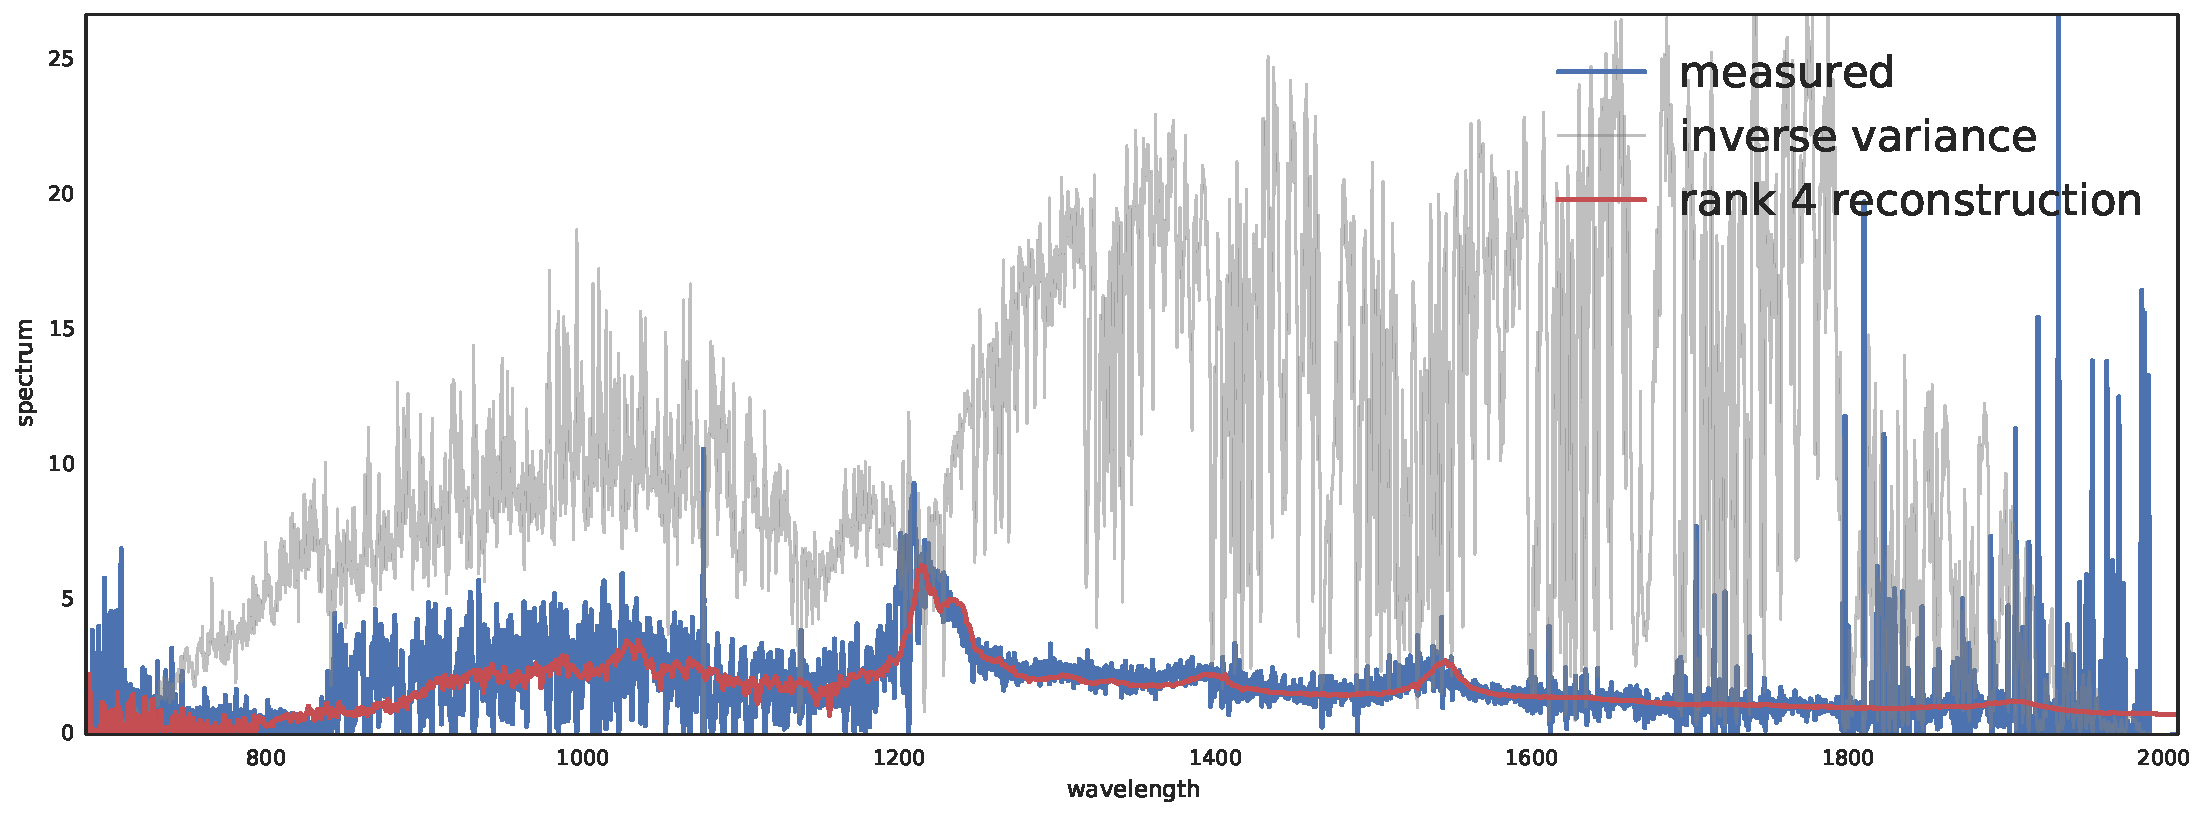
\includegraphics[width=2\columnwidth]{../figs/idx_4_rank_4_reconstruction.pdf}}
\vskip -0.2in
\caption{Top: an estimate of the maximum likelihood of the latent templates $B = \{B_k\}_{k=1}^K$.  Note the different ranges of the $x$-axis (wavelength).  Each basis function distributes its mass across different regions of the spectrum to explain different salient features of quasar spectra in the rest-frame.  Bottom: non-negative  model reconstructions of two training-sample SEDs }
\label{fig:basis}
\end{center}
\end{figure*}
%---------------

%---- TABLE, coverage --------------------------------------
\begin{table*}[ht]
\caption{Top: mean absolute and mean absolute percentage error of photometric redshift predictions with respect to spectroscopic ``ground truth''.  Bottom: number of predicted values covered by Bayesian credible intervals of varying size. }
\label{tab:error}
\vskip 0.15in
\begin{center}
\begin{small}
\begin{sc}
\begin{tabular*}{0.75\textwidth}{cccccc}
\hline
\abovespace\belowspace
  $\Delta z_{spec}$ &  $ > 0 (501)$ & $ > 1 (418)$ & $ > 2 (370)$ & $ > 3 (65)$ & $ > 4 (3)$ \\
\hline
\abovespace
MAE &  0.428 & 0.253 & 0.230 & 0.213 & 0.089 \\
MAPE &  0.397 & 0.113 & 0.090 & 0.063 & 0.022 \\
\hline
\% in $[.5, 99.5]$ &  66.5 & 77.3 & 78.9 & 81.5 & 66.7 \\
\% in $[5, 95]$    &  57.9 & 67.9 & 70.3 & 67.7 & 66.7 \\
\hline
\end{tabular*}
\end{sc}
\end{small}
\end{center}
\vskip -0.1in
\end{table*}
%------------------------------------------------------------------------------


\red{Compare $z_n$ measurements on outlier spectra with higher than $M$-sample redshift}

\red{Compare $z_n$ measurements to $r$ or $i$-band magnitude/flux level.  Can faint quasars be measured accurately as well?}

%----------------------------------------------------------------------------------
%----------------------------------------------------------------------------------
%----------------------------------------------------------------------------------
\section{Discussion}
We have presented a generative model to combine two sources of information at very different resolutions to form an estimate of the latent spectral energy distribution of quasars.  We described the details of the model, its implied structure, and a computationally tractable MCMC-based inference algorithm. 
Our experiments showed the utility of our model for the task of inferring quasar redshift from photometric data, showing that we can accurately predict and characterize uncertainty about redshift values with a small number of spectroscopic examples.  
Moreover, we showed that we can make reasonable estimates of the unobserved SED itself, from which we can make inferences about other physical properties informed by the full SED.  
 
We see multiple avenues of future work.  Firstly, we can extend the model of SED's to incorporate more expert knowledge.  One such augmentation could include a fixed collection of ``templates'' or features curated by an expert, corresponding to physical properties already known about a class of sources.  

A second goal is to place a model directly on photometric pixel observations.  Our current specification uses the output of a photometric preprocessing step, however, we would like to directly model photon counts at the pixel level and perform inference over a joint model. 
Because pixel appearance models conditioned on the SED of a source are well-known, we see this as a feasible next step. 

Our model can also be extended to include information from different photometric surveys.  Other surveys measure different ranges of the spectrum, yielding more information about the underlying SED.  Methods that incorporate photometry from different sources have been shown to improve redshift estimates \cite{brescia2013photometric}.  

Lastly, we can extend our methodology to model the SED of galaxies, which can be quite complicated.  For instance, galaxy appearances have spatial extent - photometric observations can resolve spatial features of galactic light that aren't due to the scatter modeled by a point spread function.  Furthermore, a galaxy's SED can vary \emph{spatially}, leading to far more complex models.  Models for spatial extent have been developed and applied to photometric data \cite{hogg2013replacing, regier2015}.  The combination of SED and spatial appearance modeling and computationally efficient inference procedures will lead to the automatic characterization of millions of galaxies from the enormous amounts of data available in massive photometric surveys.  

% Acknowledgements should only appear in the accepted version. 
%\section*{Acknowledgments} 
% ACM: thank dougal, dustin, jeff, jon, 
 
%\textbf{Do not} include acknowledgements in the initial version of
%the paper submitted for blind review.

%If a paper is accepted, the final camera-ready version can (and
%probably should) include acknowledgements. In this case, please
%place such acknowledgements in an unnumbered section at the
%end of the paper. Typically, this will include thanks to reviewers
%who gave useful comments, to colleagues who contributed to the ideas, 
%and to funding agencies and corporate sponsors that provided financial 
%support.  

% In the unusual situation where you want a paper to appear in the
% references without citing it in the main text, use \nocite
%\nocite{langley00}

\bibliography{../refs}
\bibliographystyle{icml2015}

\end{document} 


% This document was modified from the file originally made available by
% Pat Langley and Andrea Danyluk for ICML-2K. This version was
% created by Lise Getoor and Tobias Scheffer, it was slightly modified  
% from the 2010 version by Thorsten Joachims & Johannes Fuernkranz, 
% slightly modified from the 2009 version by Kiri Wagstaff and 
% Sam Roweis's 2008 version, which is slightly modified from 
% Prasad Tadepalli's 2007 version which is a lightly 
% changed version of the previous year's version by Andrew Moore, 
% which was in turn edited from those of Kristian Kersting and 
% Codrina Lauth. Alex Smola contributed to the algorithmic style files.  
